% Part: sets-functions-relations
% Chapter: infinite
% Section: hilberts-hotel
%
\documentclass[../../../include/open-logic-section]{subfiles}

\begin{document}

\olfileid{sfr}{infinite}{hilbert}
\olsection{Hilberts hotel}

De verzameling natuurlijke getallen is duidelijk oneindig. Maar als we
niet zomaar \emph{willen uitgaan van de natuurlijke getallen}, moeten
we eerst uitleggen wat een oneindige verzameling is, zonder die getallen
zelf te noemen. Hilbert liet in een lezing uit 1924 zien hoe dat kan.
Hij vraagt ons het volgende voor te stellen:
\begin{quote}
[\ldots] een hotel met maar een eindig aantal kamers. In elke kamer
moet precies één gast verblijven. Als de gasten dan op welke manier ook
van kamer wisselen, [maar] er nog steeds niet meer dan één persoon in
elke kamer zit, komt er geen kamer vrij. De hoteleigenaar kan zo geen
plek maken voor een gast die net aankomt [\ldots
\textparagraph \ldots]

Nu spreken we af dat het hotel oneindig veel genummerde kamers heeft:
$1$, $2$, $3$, $4$, $5$, \dots. In elke kamer verblijft precies één
gast. Zodra er een nieuwe gast aankomt, hoeft de eigenaar iedere gast
die er al was alleen naar de kamer met het eerstvolgende nummer te
verhuizen. Dan is kamer~$1$ vrij voor de nieuwe gast.
	\begin{center}
		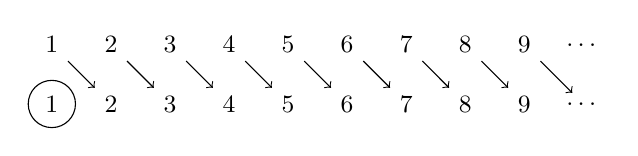
\begin{tikzpicture}[scale = .75]
		\foreach \x in {1, 2, 3, 4, 5, 6, 7, 8, 9}
		{
			\node (\x a) at (\x, 1) {\small{\x}};
			\node (\x b) at (\x, 2) {\small{\x}};
		}
		\node (dotsa) at (10, 1) {\small{\ldots}};
		\node (dotsb) at (10, 2) {\small{\ldots}};
		\draw[->] (1b)--(2a);
		\draw[->] (2b)--(3a);
		\draw[->] (3b)--(4a);
		\draw[->] (4b)--(5a);
		\draw[->] (5b)--(6a);
		\draw[->] (6b)--(7a);
		\draw[->] (7b)--(8a);
		\draw[->] (8b)--(9a);
		\draw[->] (9b)--(dotsa);
		\draw (1,1) circle (.4);
		\end{tikzpicture}
	\end{center}
	(gepubliceerd in \citealt[730]{EwaldSieg2013}; onze vertaling)
\end{quote}
Waar het om gaat, is dat Hilberts hotel oneindig veel kamers heeft. Met
zijn uitleg kunnen we vastleggen wat dat betekent. Dit is ook de aanpak
van Dedekind (we leggen Dedekind hier natuurlijk uit met een voorbeeld
dat pas veel later kwam; zijn definitie stamt uit
\citeyear{Dedekind1888}):

\begin{defn}\ollabel{defn:DedekindInfinite}
Een verzameling $A$ heet \emph{Dedekind-oneindig} precies als er een
injectie van~$A$ naar een echte deelverzameling van~$A$ bestaat. Bij
een injectie krijgen verschillende invoeren verschillende uitkomsten;
de deelverzameling is echt als zij niet de hele oorspronkelijke
verzameling is. Er ontbreekt dan minstens één element.
Anders gezegd: er is een $o \in A$ en een injectie $f \colon A \to A$
waarvoor $o \notin \ran{f}$.
\end{defn}

\end{document}